\section{Cible fonctionnelle}

    En se basant sur les dysfonctionnements identifiés précédemment et les attentes du client. Un ensemble de changement ont été prévu. Ce qui a nécessité la mise à jour de certains modèles (voir ci-dessous). Les actions précises pour la mise en place des ces changement sont décrits dans le chapitre suivant.

    \subsection{Modèle Conceptuel de Données}
        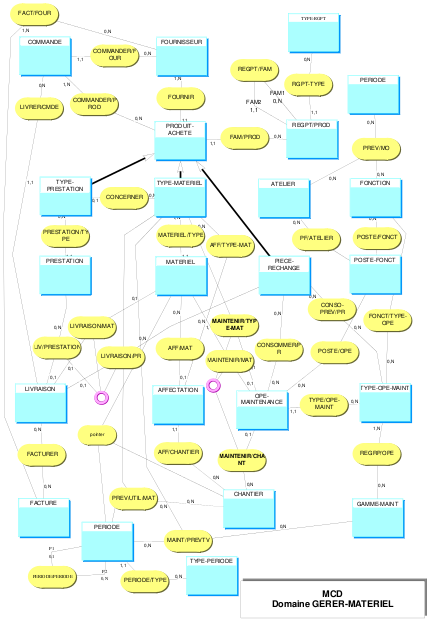
\includegraphics[width=0.9\textwidth]{img/MCD.png}

    \subsection{Modèle Conceptuel de Communication}
        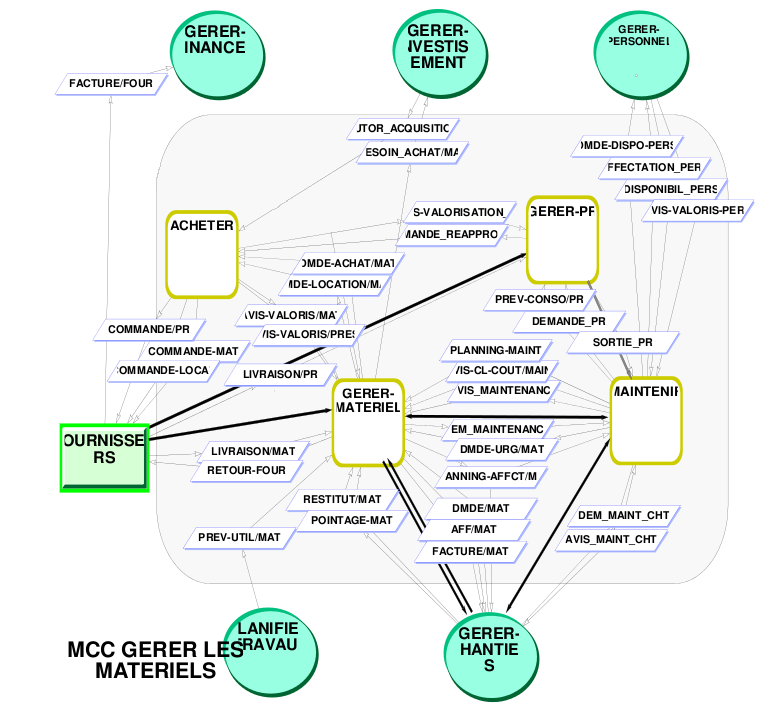
\includegraphics[width=0.9\textwidth]{img/MCC.png}

    \subsection{Diagramme de Chaine de Valeur}
        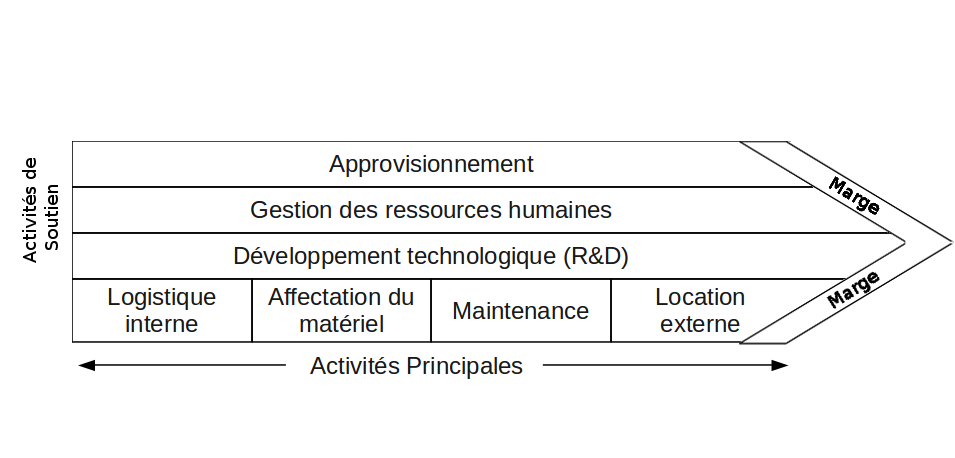
\includegraphics[width=0.9\textwidth]{img/CdV.png}

    \subsection{Activités principales}
        \begin{description}
            \item [Logistique interne]
            Les matériels et autres pièces de rechange sont ici réceptionnées des fournisseurs. Ils sont stockés jusqu'à leur affectation aux chantiers ou aux services de location externe le cas échéant.

            \item [Affectation du matériel aux chantiers]
            Les matériels demandés par les différents chantiers sont affectés à ceux-ci pour y être envoyé ultérieurement. Lorsque le matériel n’est plus utile au chantier l’ayant demandé, celui-ci est retourné au fournisseur.


            \item [Maintenance]
            Les matériels défectueux ou en panne sont traités dans des ateliers de maintenance de façon stratégique. Les pièces de rechanges les plus concernées sont disponibles sur place (l’atelier le plus proche du chantier)

            \item [Location externe]
            les matériels immobilisés sont affectés à un programme de location externe tout en gardant suffisamment de ressources pour les affectations internes.

        \end{description}

    \subsection{Activités de soutien}
        \begin{description}
            \item [Approvisionnement]
            GSTP doit se fournir et donc acheter des matériels et pièces de rechanges ainsi que d’autres biens et services. Le but de cette fonction est d'obtenir le plus bas prix pour la meilleure qualité pour tous ces achats. Une gestion optimisée des fournisseurs est appliquée si bien que la proximité géographique du fournisseur est prise en compte afin de réduire les coût de transport et les délais de livraison.
            \item [Gestion des ressources humaines]
            Il est important d’avoir dans toute entreprise un service de Gestion de ressources humaines afin de mobiliser et développer les ressources humaines pour une plus grande performance de l'organisation. Ce service permet d’améliorer la communication transversale au sein de l’entreprise, tout en faisant respecter son organigramme.

            \item [Développement technologique (R\&D)]
            Les technologies sont des sources importantes d'avantage concurrentiel. Les entreprises ont besoin d'innovation pour réduire leurs coûts, se protéger et maintenir leur avantage concurrentiel. Ceci englobe le développement technologique, les activités marketing internet, la gestion des relations avec les clients .

    \end{description}
